\section{Introduction}\label{sec:intro}
An important question plaguing machine learning \cite{BenAli-1,Lecun,BenAli-2,Aliresponse,Mickens} is:
\begin{center}
\textbf{\emph{Is Deep Learning Alchemy?}}
\end{center}
The \emph{alchemy} question can further be broken down into sub-questions/issues/gaps as listed below. 

1. \emph{Training:} Despite a \emph{non-convex} loss surface, why is it possible for stochastic gradient descent (SGD) (and its variants) to achieve zero training error in standard deep neural networks (DNNs)?

2. \emph{Generalisation:} Standard DNNs are \emph{over-parameterised}, yet, when trained on data with true labels we observe good test performance. Does understanding deep learning require rethinking generalisation? \cite{ben}

3. \emph{Depth:} Approximation results show that more depth is better \cite{depth1,depth2}, i.e., deeper models can approximate more complicated target functions better than shallow models. Yet, when training on standard datasets, increasing the depth beyond a point adversely affects both training and test performance \cite{resnets}. This situation can be remedied by using \emph{skip connections} giving rise to residual neural networks. However, why increasing depth beyond a point hurts standard DNNs is still not understood satisfactorily. 

4. \emph{Depth vs Width:} Wider models \cite{wide1,wide2,wide3} have also been quite successful. While increasing either depth or width causes an increase in the number of model parameters, the trade-off between width and depth is not clearly understood.

5. \emph{Functionality:} The roles of the basic parts namely weights and activation have not been clearly understood.

6. \emph{Uninterpretablity of Learnt Representation:} The commonly held view of feature learning is that lower level features are learnt in the initial layers and as one proceeds in depth more sophisticated features are learnt in the higher levels and the final layer learns a linear model in the features given by the output of the penultimate layer. However, there is no straightforward way to interpret the features learnt in the hidden layers.

7. There is a gap between \emph{universal approximation results} which characterise the class of functions representable by DNNs and \emph{practical} DNNs that are trained using SGD (and variants) starting from randomly initialised weights. Further, the performance of DNNs are evaluated on standard datasets such as MNIST and CIFAR-10. 

\textbf{Our Work:} To address the aforementioned questions/issues/gaps, we propose a \emph{pedagogical nugget} of ``simple theorems, and simple experiments" \cite{Aliresponse} based on two prior works namely (i)\emph{duality} and (ii) \emph{neural tangent kernel} (NTK).  We now place our work in relation to prior works on (i) NTK, (ii) Duality (see \Cref{fig:related}).

\subsection{Duality and Neural Tangent Kernel}

\textbf{Neural Tangent Kernel:} One of the approaches to understand the training and generalisation of a DNN is to study kernels associated with the DNN. Two important kernels associated with a DNN are its \emph{Conjugate Kernel (CK)/ Gaussian Process Kernel (GPK)} and the so called \emph{Neural Tangent Kernel (NTK)} . The CK is the Gram matrix of the features obtained at the penultimate layer output of the DNN. The NTK is Gram matrix of the Jacobian output of the DNN with respect to its weights. As width approaches to infinity, both the CK and the NTK converge to (their corresponding) limiting deterministic matrices. It has been shown that training the last layer of the infinite width DNN (known as \emph{lazy training}) is equivalent to a kernel method with the limiting CK and training all the layers of an infinite width DNN (known as \emph{full training}) is equivalent to a kernel method with the limiting NTK. Thus training and generalisation of infinite width DNNs boils down to the properties of the limiting deterministic kernel matrix. On CIFAR-10, the test accuracy of CK, NTK and standard DNN (all of three of them use convolution layers) is as follows:
\resizebox{\columnwidth}{!}{
\begin{tabular}{ccc}
CK & NTK & Standard\\
\cite{convgp} & \cite{arora2019exact} &  DNN\\
$\approx 67\%$&$\approx 77\%$&$80\%$ and above
\end{tabular}
}

The NTK performs better than the CK as well as other prior pure kernel based methods \cite{arora2019exact}. However, standard finite width DNN (with convolutional layers) still outperforms its infinite width NTK counterpart. As a result, NTK was not fully adequate to explain DNNs.
\begin{figure}
\resizebox{\columnwidth}{!}{
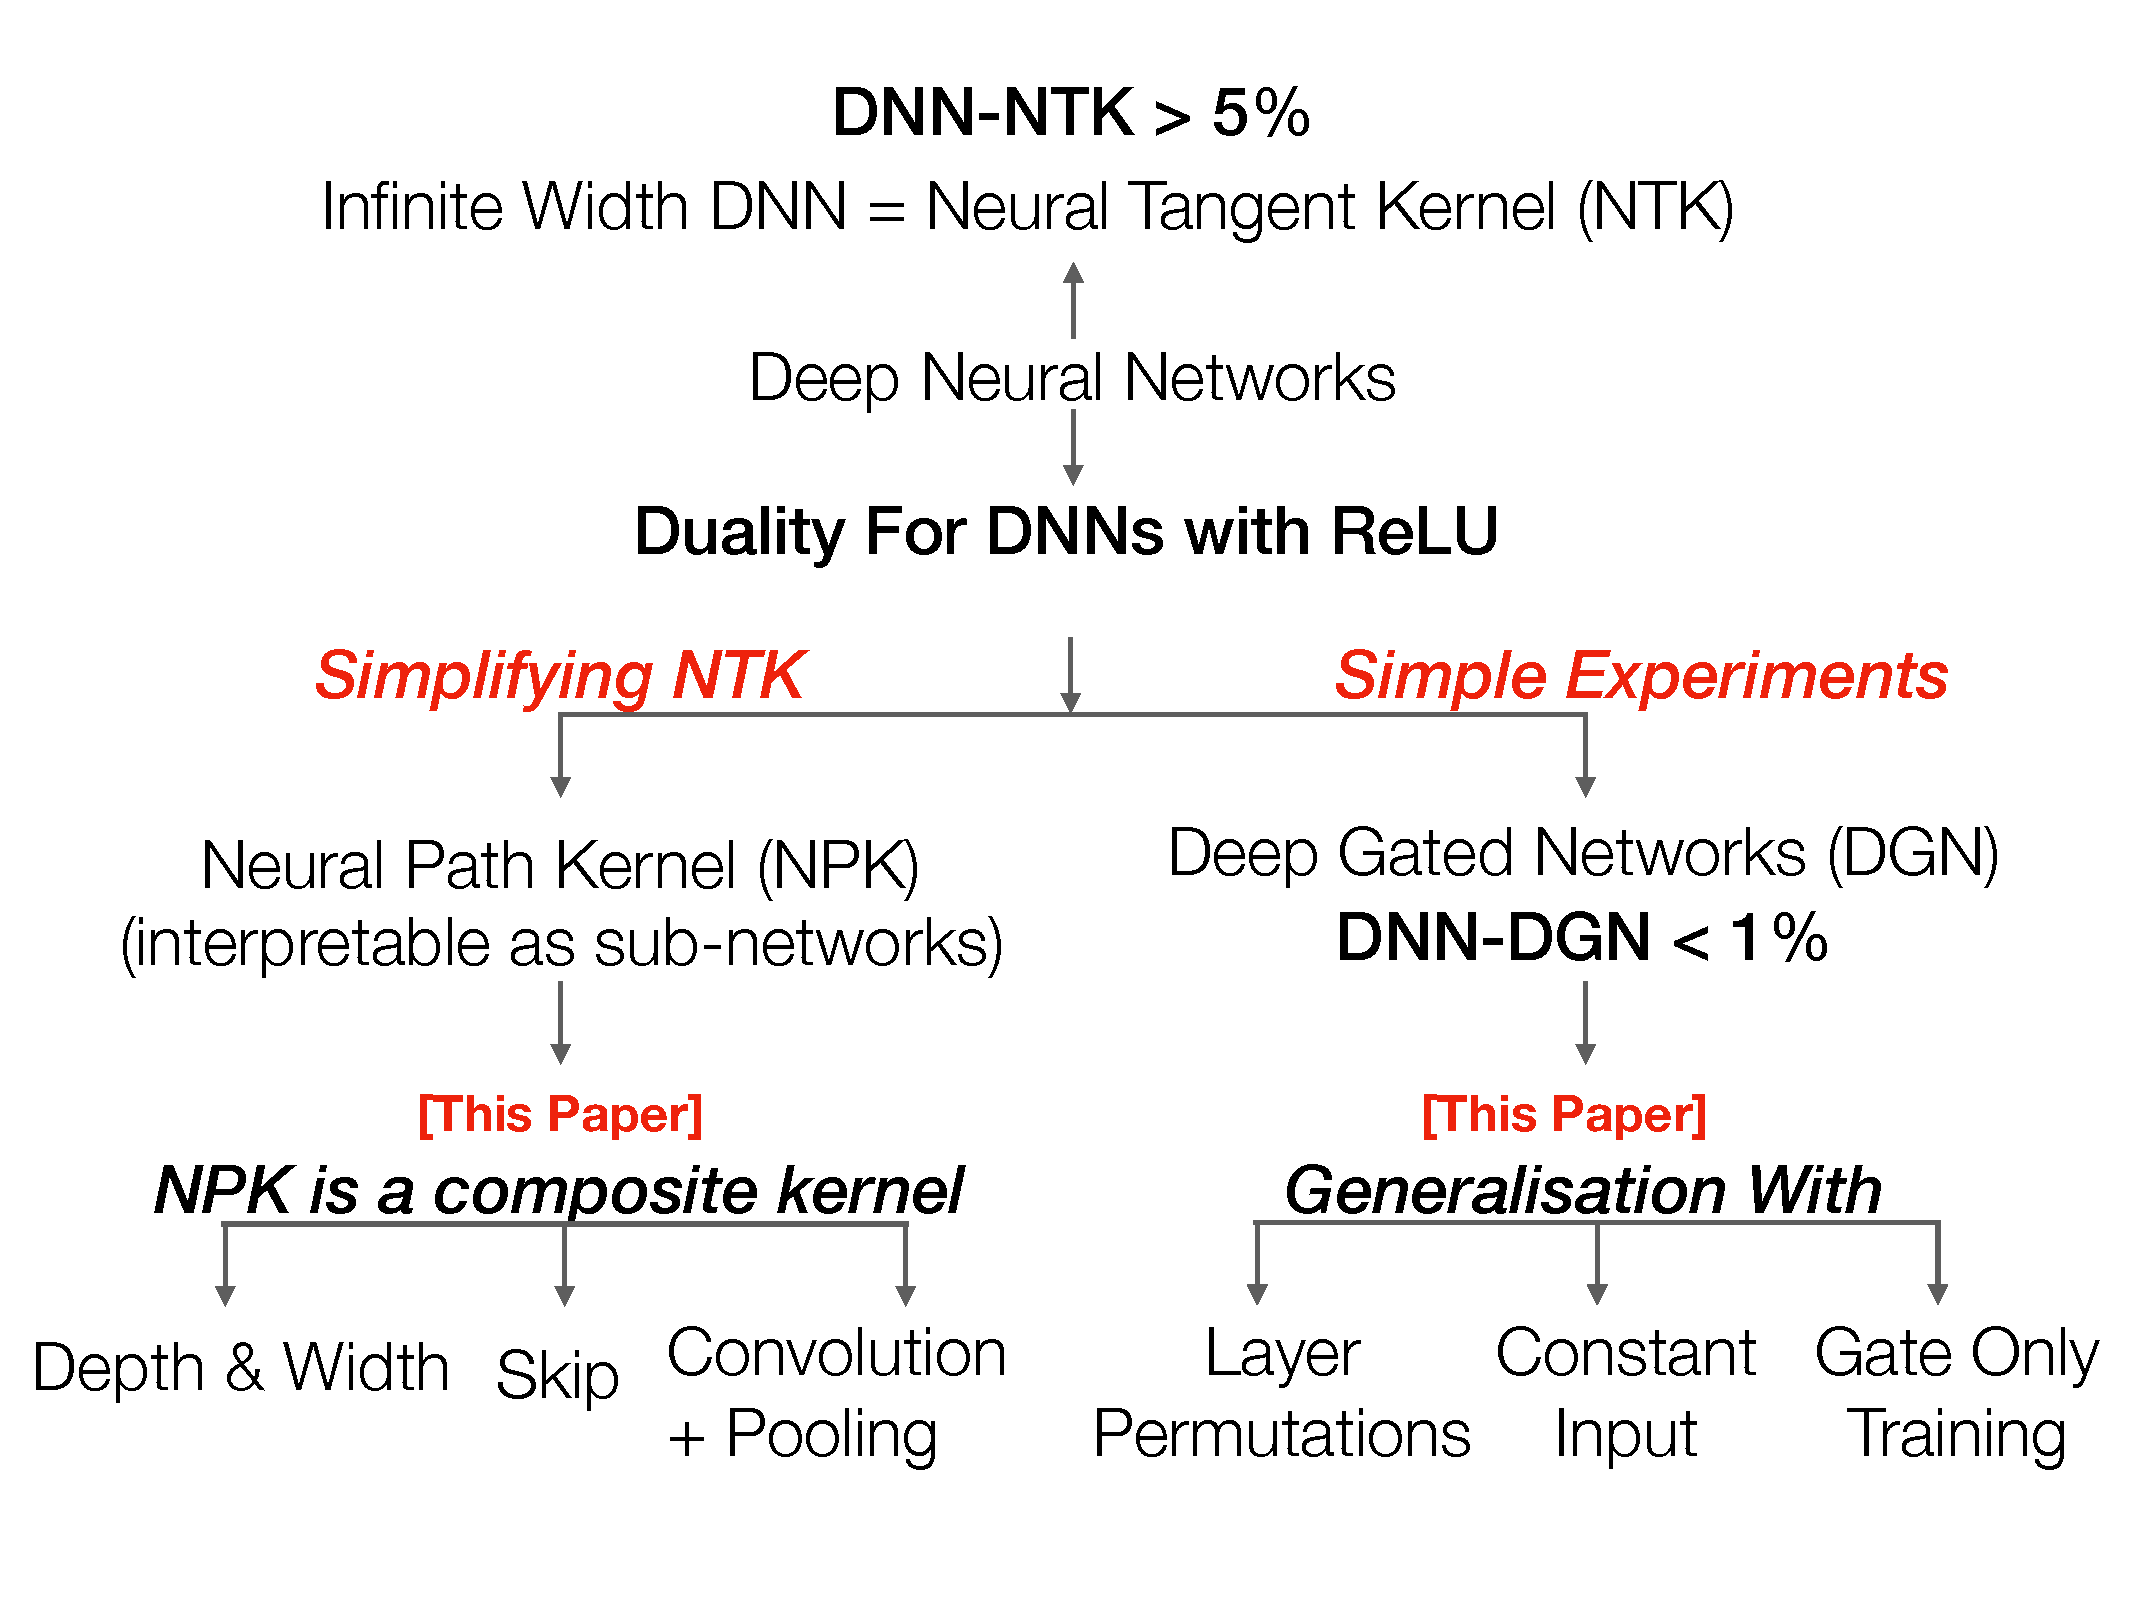
\includegraphics[scale=0.25]{figs/related.pdf}
}
\caption{This paper in relation to (i) NTK, (ii) Duality.}
\label{fig:related}
\end{figure}

\textbf{Duality and Simple Experiments:} In their recent work \cite{npk} proposed a dual approach to analyse DNNs with the rectified linear units (ReLUs). They exploited the special gating property of ReLU to devise a simple experimental setup called the deep gated network (DGN). In a DGN, the gates and the weights are held in separate networks as opposed to a DNN in which gates and weights are in the same network (see \Cref{fig:dgn}). They showed experimentally that:

\begin{figure}
\centering
\resizebox{\columnwidth}{!}{
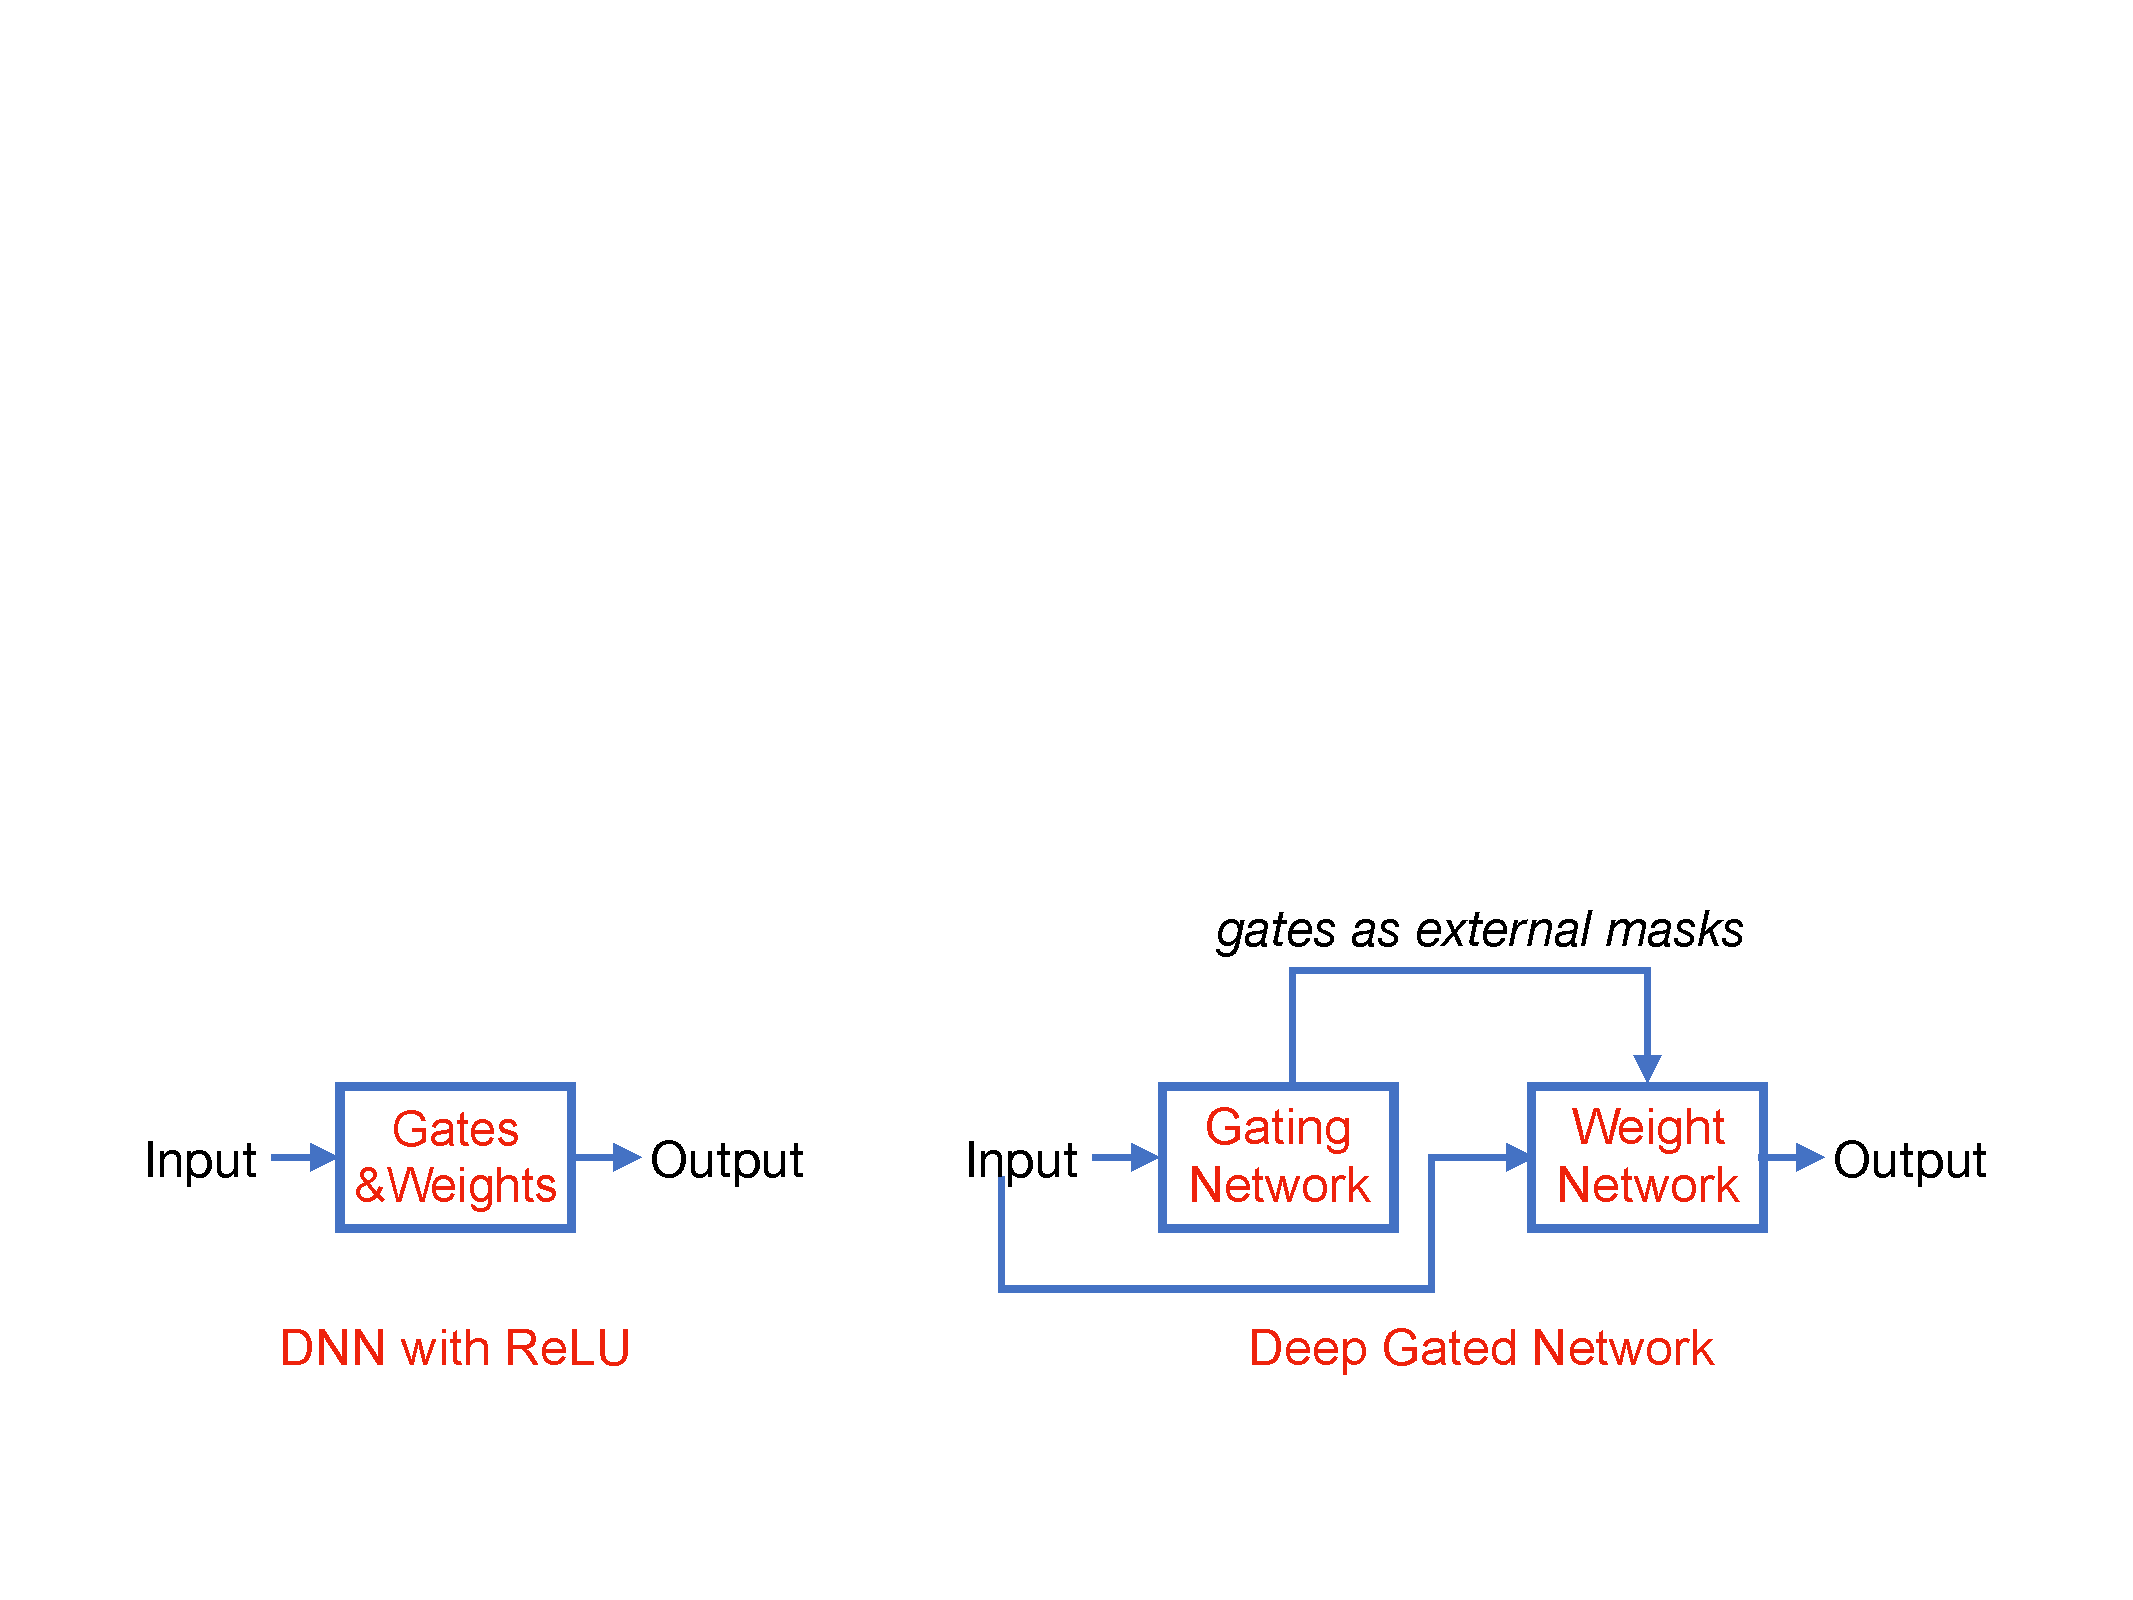
\includegraphics[scale=0.25]{figs/dnn-dgn.pdf}
}
\caption{DNN vs DGN.}
\label{fig:dgn}
\end{figure}
$1.$ \emph{Most information is in the gates:} By using just the gates of a pre-trained DNN (by letting it to be the gating network), the weight network can be trained to match the test performance (within $1\%$ ) of the DNN.

$2.$ \emph{Learning in gates} is the difference between finite width DNN and the infinite width NTK.  

\textbf{Duality simplifies NTK:} \cite{npk} showed that in a DGN:$\text{NTK}=\text{NTK}^{\text{fixed-gate}}+\text{NTK}^{\text{gate-learn}}$, where $\text{NTK}^{\text{fixed-gate}}$ is the kernel corresponding to learning of the weights with the gates fixed and $\text{NTK}^{\text{gate-learn}}$ is the kernel corresponding to learning of gates themselves. Further, $\text{NTK}^{\text{fixed-gate}}$ simplifies into a \emph{neural path kernel} (NPK), a kernel which is solely dependent on the information stored in the gates.



\subsection{Our Contributions}
The overall picture of duality and NTK results can be summarised  as follows: (i) training and generalisation of infinite width DNNs is explain by the NTK \cite{arora2019exact,cao2019generalization}, (ii) the difference between finite width DNNs and infinite width DNNs is explained by learning in gates \cite{npk}, (iii) ReLU activation has a special role, i.e., they are gates, (iv) the primary role of the weights is to trigger the ReLU on/off. In this work we complete the picture by explaining the roles of width, depth, skip connections and convolutional layers with pooling.  The theoretical and experimental contributions are listed as under.

\FloatBarrier
\begin{figure}[h]
\centering
\resizebox{\columnwidth}{!}{
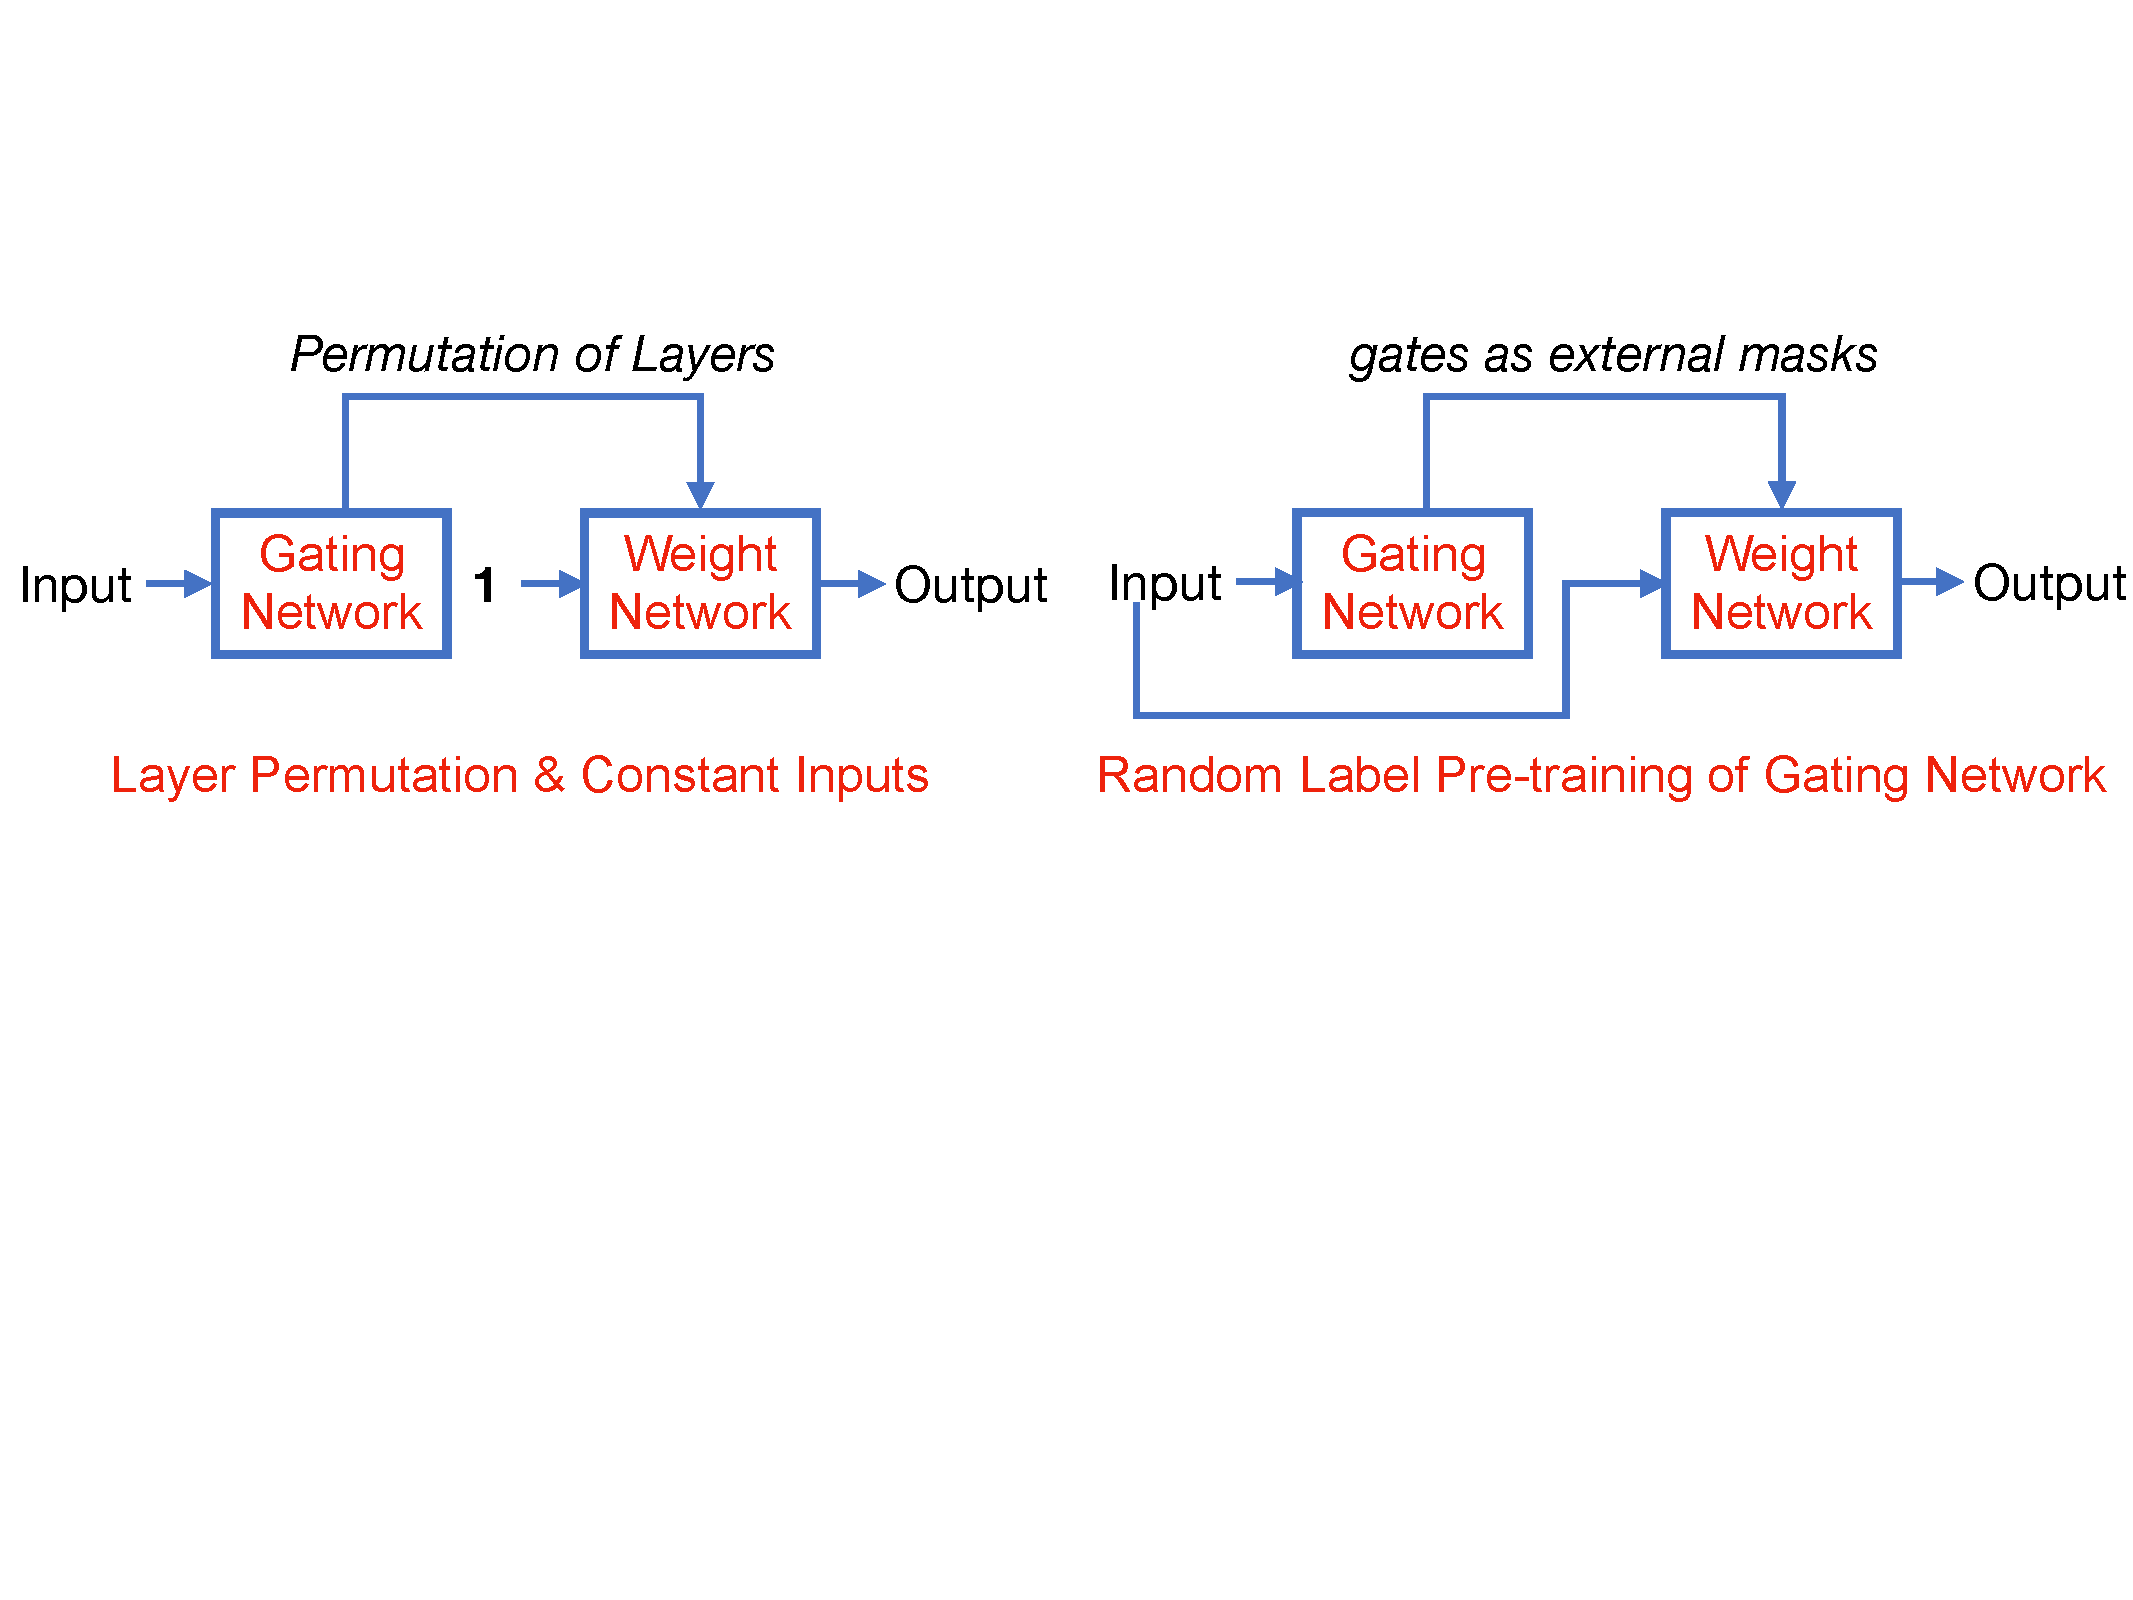
\includegraphics[scale=0.25]{figs/permute.pdf}
}
\end{figure}



\begin{table}
\begin{tabular}{ccccccccc}\hline
Primal & A & B & C& D & E& F & G & H\\ \hline
Kernel & A & B & C& D & E& F & G & H\\ \hline
Dual-View& A & B & C& D & E& F & G & H\\ \hline
\end{tabular}
\end{table}



\textbf{Theoretical Results:} We show that the NPK has a \emph{composite structure}, whose basic atomic units are the \emph{gates}. Specifically,

$\bullet$ \emph{Fully Connected DNN (FC-DNN):} In this case, the NPK involves a \emph{ Hadamard product of base kernels} structure. Here the most basic unit is the gate.  stacking ReLUs widthwise in a layer gives rise to a base kernel which measures the \emph{average} number of triggered ReLUs; stacking layers depthwise gives rise to a \emph{Hadamard product}. This result explains the roles of \emph{width and depth}.

$\bullet$ \emph{Residual networks with skip connections:} In this case, the NPK involves a  \emph{ sum of Hadamard product of base kernels} structure. This result explains the role of skip connections.

$\bullet$ \emph{Convolutional layers with pooling:} In this case, the NPK  has a  \emph{rotational invariant} structure. This result explains the role of convolutions and pooling from a kernel standpoint.

\textbf{Experimental Results:} We collect more supporting evidence for the claim \emph{most information is in the gates}. In particular, our results show that the standard view that hidden layer outputs is a red-herring and the actual feature learning happens in the gates. To bolster our case, we build combinatorially many models by (i) permuting the order of the layers when we apply them as external masks and providing a tensor with all entries $1$ instead of the input image. 

\textbf{Message:} The primal \emph{layer-by-layer} and the dual \emph{path-by-path} views of computations complement each other. While the primal computations is used in \emph{actual} training and our results suggest that dual view is quite for understanding. 

\begin{comment}
 We consider deep neural networks (DNNs) with \emph{rectified linear units} (ReLUs). For such DNNs, we propose a \emph{pedagogical nugget} ``simple theorems, simple experiments" \cite{Aliresponse} by combining \emph{neural tangent kernel} (NTK) and \emph{dual view}. Our aim is to explain training, generalisation, roles of weights/activation/width/depth/convolutions with pooling/skip connections. Training and generalisation of infinite width DNN 


In this paper, we make two major contributions using the lens of dual view. Firstly, we show that the NPK has a \emph{compositional} structure. The results are listed below.

$\bullet$ \emph{Fully Connected DNN (FC-DNN):} In this case, the NPK involves a \emph{ Hadamard product of base kernels} structure. Here the most basic unit is the gate.  stacking ReLUs widthwise in a layer gives rise to a base kernel which measures the \emph{average} number of triggered ReLUs; stacking layers depthwise gives rise to a \emph{Hadamard product}. This result also explains the roles of \emph{width and depth}.

$\bullet$ \emph{Residual networks with skip connections:} In this case, the NPK involves a  \emph{ sum of Hadamard product of base kernels} structure.

$\bullet$ \emph{Convolutional layers with pooling:} In this case, the NPK  has a  \emph{rotational invariant} structure.

Our second major contribution is an ablation study to argue that the standard view that hidden layer outputs is a red-herring and the actual feature learning happens in the gates. To bolster our case, we build combinatorially many models by,

1. permuting the order of the layers when we apply them as external masks,

2. providing a tensor with all entries $1$ instead of the input image. 

We observe in our experiments that the performance is robust to such combinatorial variations.

We also show experimentally how training with random labels affects the gates, and experimentally verify how skip connections improve the conditioning of the underlying NTK.
\end{comment}
\subsection{Organisation}
\subsection{Notation}